\begin{frame}{Global Picture}
\centering
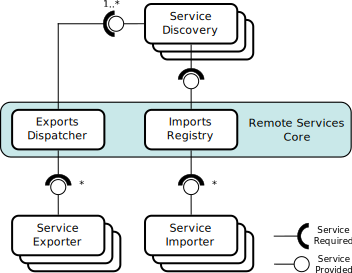
\includegraphics[height=.8\textheight]{../imgs/rs_arch}
\end{frame}

\begin{frame}{Remote Services Services}
\begin{exampleblock}{Note}
All services names are declared in \texttt{pelix.remote}
\end{exampleblock}

\begin{block}{Core Services}
\begin{small}
\begin{tabular}{rp{.55\textwidth}}
\texttt{\scriptsize SERVICE\_DISPATCHER} & Read-only access to the list of export endpoints \\
\texttt{\scriptsize SERVICE\_DISPATCHER\_SERVLET} & Utility methods for HTTP-based discovery \\
\texttt{\scriptsize SERVICE\_REGISTRY} & Write-only access to the list of import endpoints \\
\end{tabular}
\end{small}
\end{block}

\begin{block}{Import/Export Services}
\begin{small}
\begin{tabular}{rp{.45\textwidth}}
\texttt{\scriptsize SERVICE\_EXPORT\_PROVIDER} & Notified by the dispatcher to create export endpoints \\
\texttt{\scriptsize SERVICE\_EXPORT\_ENDPOINT\_LISTENER} & Notified of new export endpoints \\
\texttt{\scriptsize SERVICE\_IMPORT\_ENDPOINT\_LISTENER} & Notified of new import endpoints \\
\end{tabular}
\end{small}
\end{block}
\end{frame}

\begin{frame}{Endpoint creation sequence}
\begin{small}
\begin{block}{Service export/import}
The \texttt{Dispatcher} is notified of a service to be exported (after its registration or update), notifies the exporters and notifies the discovery services about the created endpoints.
\end{block}
\end{small}

\vspace{2ex}

\centering
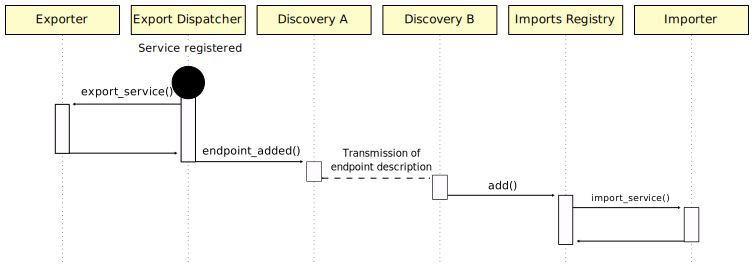
\includegraphics[width=\textwidth]{../imgs/rs_sequence}
\end{frame}

\begin{frame}{How to export a service?}
\begin{block}{How it works}
\begin{enumerate}
\item Services with export properties are detected by the dispatcher
\item The dispatcher notifies the export services
\item Each exporter can create an \texttt{ExportEndpoint}
\item The dispatcher notifies the discovery services
\end{enumerate}
\end{block}

\begin{block}{Export properties}
\begin{tabular}{rl}
\texttt{\small service.exported.interfaces} & List of exported interfaces \\
\hline
\texttt{\small service.exported.configs} & List of allowed export protocols \\
\end{tabular}
\end{block}
\end{frame}

\begin{frame}{How is a service imported?}
\begin{block}{How it works}
\begin{enumerate}
\item A discovery service detects a new service
\item The discovery service notifies the Imports Registry
\item The ImportRegistry notifies the import services
\item Each import service can register a proxy as a local service, with import properties
\end{enumerate}
\end{block}

\begin{block}{Imported service properties}
\begin{tabular}{rl}
\texttt{\small service.imported.interfaces} & List of exported interfaces \\
\hline
\texttt{\small service.imported.configs} & List of allowed export protocols \\
\hline
\texttt{\small endpoint.framework.uuid} & UUID of the host framework \\
\hline
\texttt{\small endpoint.service.id} & Service ID in the host framework \\
\end{tabular}
\end{block}
\end{frame}


\begin{frame}{Supported protocols}
\begin{exampleblock}{Java compatibility}
A Java implementation of iPOPO Remote Services is available as the \href{https://github.com/isandlaTech/cohorte-remote-services}{Cohorte Remote Services} project.
\end{exampleblock}

\begin{small}
\begin{columns}[t,onlytextwidth]
\column{.4\textwidth}
\begin{block}{Discovery}
\centering
\begin{tabular}{ll}
\textbf{Protocol} & \textbf{Specification}\\
Multicast & iPOPO specific\\
MQTT & iPOPO specific\\
ZeroConf & Standard\\
\end{tabular}
\end{block}

\column{.55\textwidth}
\begin{block}{Transport}
\centering
\begin{tabular}{ll}
\textbf{Protocol} & \textbf{Specification}\\
XML-RPC & Standard\\
JSON-RPC & Standard\\
Jabsorb-RPC & from the Jabsorb project\\
MQTT-RPC & iPOPO Specific\\
\end{tabular}
\end{block}
\end{columns}
\end{small}
\end{frame}
